% \documentclass[10pt,a4paper,twocolumn]{article}
\documentclass[10pt,a4paper]{article}
\usepackage[utf8]{inputenc}
\usepackage[T1]{fontenc}
%\usepackage{gentium}
\usepackage[labelfont=bf]{caption}
\usepackage{float}
\usepackage{mathptmx} % Use Times Font
\usepackage{amsmath}
\usepackage{tabularx}
\usepackage{amsfonts}
\usepackage{graphicx} % Required for including pictures
\usepackage{hyperref} % Format links for pdf
\usepackage{biblatex}
\addbibresource{references.bib}
\usepackage{booktabs} % Used so that tables generated by pandas
                      % to_latex() work correctly
\usepackage{multicol}
\frenchspacing % No double spacing between sentences
\usepackage[margin=1in]{geometry}

\usepackage[all]{nowidow} % Tries to remove widows
\usepackage[protrusion=true,expansion=true]{microtype} % Improves typography, load after fontpackage is selected

\usepackage{lipsum} % Used for inserting dummy 'Lorem ipsum' text into the template

\title{failing to predict en passant :(}
\author{Leon Lee and Lila Marshman}

\begin{document}

\maketitle

%% INSTRUCTIONS:
%%
%% 1. Create your own copy of this Overleaf project. You can either edit your report
%% using:
%%
%%    a. Overleaf professional, a collaborative LaTeX editor. You can click
%%       "Copy Project" from the Overleaf menu to create a version where you have
%%       read and write permissions. See the following for documentation:
%%       https://www.overleaf.com/edu/edinburgh and
%%       https://uoe.sharepoint.com/:f:/r/sites/digitalskillsandtraining/Shared%20Documents/LaTeX/LaTeX%20for%20Beginners%20using%20Overleaf?csf=1&web=1&e=cPqTI3
%%
%%    b. A LaTeX editor on your PC. For this option, you can download the source
%%       of this project as a zip (via the Overleaf menu).
%% 
%% 2. Please rename this file fds-project-option-1.tex, 
%% fds-project-option-2.tex, or fds-project-option-3.tex, depending on
%% which project option you are doing. When you submit, please submit
%% the PDF file with the corresponding name.
%% 
%% 3. Please keep the section and paragraph headings as they
%%    are. You should delete all the text within the headings, e.g.
%%    the text that says "What is the area of this data science
%%    study, and why is it interesting to investigate" and the
%%    bullet points. Keeping the headings makes the report a lot
%%    easier for the markers to read, and making things easy for
%%    markers is always beneficial.
%%
%% 4. The word limit for the Overview section is mandatory. For the
%% other sections word limits are suggested.
%%
%% 5. The page limits must be strictly adhered to, and depend on if
%% you are working individually, in pairs or in threes:
%%
%%   - Individual: 6 pages 
%%   - Pairs: 8 pages 
%%   - Threes: 10 pages 
%%
\section{Overview}
% 250 words maximum
Online chess sites receive a huge amount of game data from large volumes of users accessing and playing on their sites. Many have large player bases, representing a huge variety in player Elo scores (a number corresponding to skill level). We used data from games played on the online chess website Chess.com to analyse the relevancy of players' Elo in a chess game. We used a logistic regression model to investigate the effect of the difference in Elo on winning a game. Following from this, by using an exponential function "Temptation", we were able to visualise a player's likelihood of playing a specific chess tactic called \textit{en passant} across three different categories of Elo. We then attempted to predict a player's Elo using the context of said en passant move. By analysing computer generated evaluations of the state of the game preceding the move, and by using Temptation as a hyperparameter for a predictive model, we attempted to utilise PCA and a K-Nearest Neighbour algorithm to classify users into three classes of Elo. To evaluate the model we calculated various metrics (accuracy, precision, recall, F1 score). [Lila Talk about evaluation and results]\newline
All decimal values in this report are provided to 4 decimal places.

% Visualisations of ...
% Statistical techniques used ...
\begin{multicols}{2}
[
\section{Introduction}
]
% Suggested 400 words

\paragraph{Context and motivation}

Online chess sites such as Chess.com allow users to play with friends or strangers, offering a wide variety of chess variants and time controls to play with. Online chess' rise in popularity follows the increase in free time during the COVID-19 pandemic lockdowns, the popularity of Netflix's show 'The Queen's Gambit', and world-ranking players streaming the game on Twitch \cite{The2020ChessBoom} With a sudden increase in online players comes an increase in publicly available game data - this provides a perfect opportunity for an investigation into player's skill (measured by Elo points). In this study, we explore the impact of a player's skill level on a game's direction and patterns in the play styles of players at different Elos. \newline

The particular play style we explore in this study is the context surrounding an \textit{en passant} chess move. Typically, chess tactics are something you aim for, therefore there is the natural assumption that a higher-ranked player would be able to set up certain tactics more consistently than a lower Elo one. One exception to this is the move \textit{En passant}. It is an incredibly situational move, and it heavily relies on a player's opponent to move a certain way for a player to be able to play it in the first place. In the chess scene, particularly in the online chess community, \textit{en passant} has gained a cult-like following\cite{EnPassant}. It's become a popular running joke amongst players to always capture via \textit{en passant} when given the chance, even if this puts them in a worse position than having not chosen that move. Losing an online game results in your Elo rating decreasing, thus most would expect highly rated players to not risk a bad game position, hence not capture \textit{en passant} unless it's beneficial. In this study we explore whether we can use the context surrounding an \textit{en passant}-allowed board state to predict whether a player falls into the low, medium, or high Elo category. \newline

Insight into these areas, particularly if the second investigation proves Elo is predictable from move contexts, may be useful in determining how players in the past compare to today's players. There is much speculation on how historical chess champion Bobby Fischer would compare to current world champion Magnus Carlsen \cite{BobbyFischerVsMagnusCarlsen}, thus if we are able to predict a modern-day Elo for Fischer by inputting his play style information into a model trained on modern games, we may find evidence suggesting how he'd compare.

\paragraph{Previous work}

Brief description of any previous work in this area (e.g., in the
media, or scientific literature or blogs).

LILA REMOVE THIS (just here so I can remember tomorrow):
% https://books.google.co.uk/books?hl=en&lr=&id=-tlGEAAAQBAJ&oi=fnd&pg=PT8&dq=chess+elo+rating+and+winning+game&ots=88A7EmxI8j&sig=ZsdoYnjPizF3OONpEcV2iCoHhEA#v=onepage&q=chess%20elo%20rating%20and%20winning%20game&f=false

% https://scholarlypublishingcollective.org/uip/ajp/article-abstract/118/1/29/257902/A-Psychometric-Analysis-of-Chess-Expertise

% https://en.chessbase.com/post/elo-meter-the-test-that-calculates-your-elo

A book by Holding \cite{PsychologyOfChessSkill} suggests that Elo ideally Elo follows a normal distribution with a mean of $1,500$ and a standard deviation of $200$ - however this fluctuates as the population of rated chess players over time. Holding \cite{PsychologyOfChessSkill} proposes that if Elo follows this distribution exactly, a player rated at the mean has a $0.25$ chance of winning against players rated at $1,700$, and a $0.1$ chance of winning against players rated $1,875$, though it is unclear how these probabilities were calculated. This implies there is some known association between comparative Elo and winning, though no further explanation on this is given.

An article published on the website 'Towards Data Science' \cite{HowMuchDoesEloMatter} found a relationship between Elo disparity and winning within a range of $\pm 50$ Elo points difference, but outside of this range an increase in Elo had little effect on increasing or decreasing the probability of a win. \cite{HowMuchDoesEloMatter} created a logistic regression model to predict winning probability for data points within the $\pm 50$ Elo points difference. They demonstrated there was a correlation, however, they do not explore logistic regression coefficients, interpret their visualisations, or evaluate their model any further than stating their AUC metric is "not bad". This provides the opportunity for us to explore data outside the $\pm 50$ Elo difference range, as well as running hypothesis tests and interpreting regression coefficients to further justify \cite{HowMuchDoesEloMatter}'s findings.
There is no literature directly studying the relationship between a player's response to \textit{en passant} moves and their Elo.
\paragraph{Objectives}

Our goals in this study are to investigate whether there is a correlation between a player's Elo, and the moves they play in a game. In our case we are focusing on the move \textit{en passant}, and a player's willingness to play the move if an opportunity presents itself. We will first take a bird's eye view of the overall effects of Elo, and investigate whether a significant gap in Elo affects the chances of winning. Then, we will analyse games containing the move \textit{en passant}, and through the context of the board state try and determine a player's Elo, and indirectly, their chance of winning.
% What questions are you setting out to answer?

\section{Data}
% Suggested 300 words

% Who created the dataset(s)?  How you have
% obtained it (e.g., file or web scraping), and do the T\&Cs allow you
% to use obtain the data for the project?

\paragraph{Data provenance}
We obtained our data from Kaggle.com \cite{Kaggle}, where they provided a dataset of over 60,000 games of chess taken from Chess.com. The User Agreement on Chess.com states that you are not allowed to data mine \cite{ChessT&C}, but in this case the dataset was extracted using the Chess.com API so it complies with their regulations.

% Description of the data, e.g. variables
% in each table, number of records.
\paragraph{Data description}
The dataset records $66,879$ games of chess that took place on Chess.com with varying game modes, time classes, and levels of players. Information about each player is provided, i.e. the usernames, Chess.com profiles, and Elo rating during the match. Information about the game is also provided, i.e. the result, information about the time rules, whether it was rated, and the final chess board in a notation called "FEN". The final column is called the PGN (Portable Game Notation) - a column in a standard format to be easily read by other chess analysers. Within the PGN, there includes a list of the moves that took place during the game. Using this we can simulate and replay exactly how the game was played, and provide further analysis.


\paragraph{Data processing}
For both investigation questions, we removed alternate game modes that were not standard chess (for example, 'Chess960', and all game records if they contained any NaN values. We removed games where the game terminated early by using two filters: determining no major pieces had been moved (by reading the top row of the 'FEN', and removing games with less than 10 total moves (5 per player). We believed any games in these two categories would not be useful to the data analysis. Additionally, we removed games from the 'daily' time class. This was due to these records' 'PGN' column being structured in a different format, meaning daily games would have needed to be analysed separately from other modes. Additionally, unlike the rest of the remaining games, 'daily' games had no time pressure on players - thus removing these removes the chance that time pressure may have affected the results as a confounding variable. Due to this, and the fact there was only a small amount of 'daily' games ($\sim9.2\%$ of total games), we removed these from the dataset.\newline

For the first investigation, we required a binary outcome (winning or losing) in order to use logistic regression, thus we additionally excluded all games which ended in a draw or other indeterminate end-states. \newline

For our second investigation, we utilised various external libraries to assist in defining k-NN hyperparameters. Using the \textit{python-chess} library \cite{python-chess}, we parsed the "PGN" field to filter out games that didn't include an \textit{en passant} opportunity ($n=5074$), and highlight games where an \textit{en passant} move actually occurred ($n=1563$). We then used \textit{Stockfish}\cite{StockFish}, an open-source chess game engine, to evaluate how much of an advantage from an initial board state a player would gain from the following moves: a Stockfish calculated best move, the move the player decided to make, and finally the relevant \textit{en passant} capture. These scores were added to the dataframe. All non-numerical data were converted to numerical data by assigning numerical categories. This was important for standardising the data, performing a PCA and creating the k-NN model.\newline


\begin{figure*}[p]
  \centering
  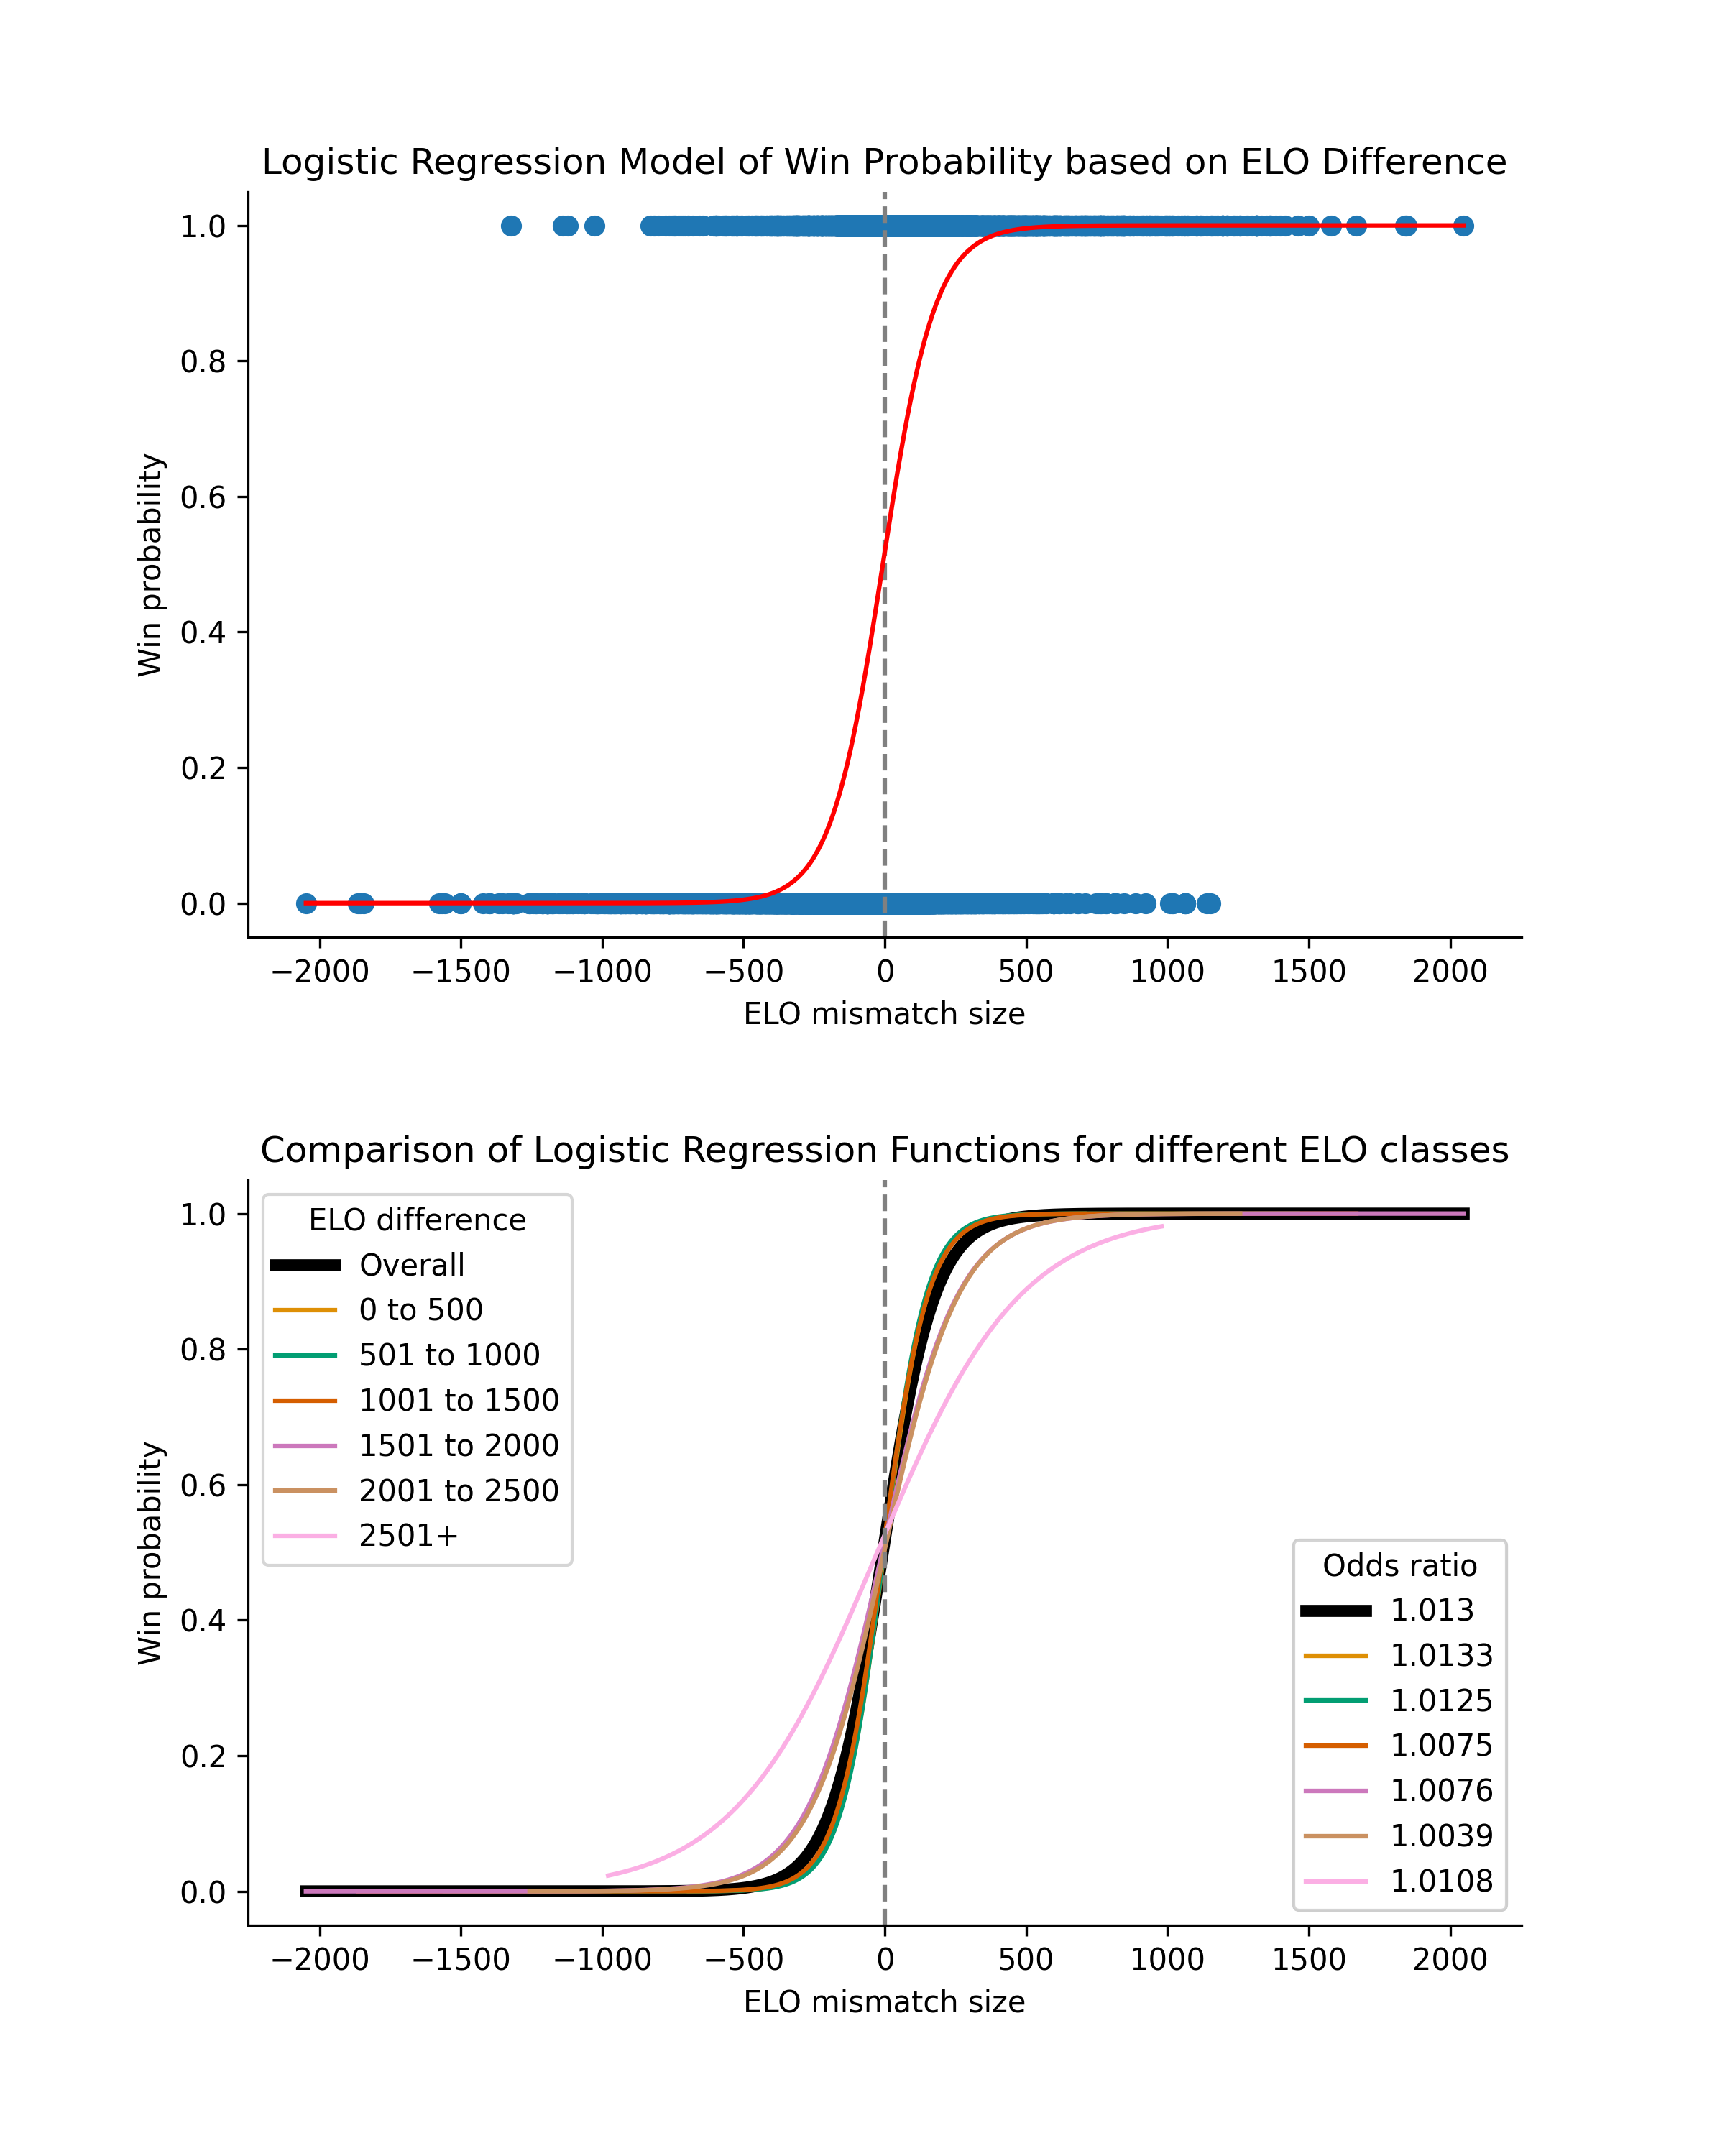
\includegraphics[width=\textwidth]{report/images/log_regression_dual.png}
  \caption{Subplot 1: Each datapoint represents how many Elo points a player is than their opponent during a game, and whether they won (1) or lost (0). The standard logistic function is plotted in red. 'Elo mismatch size' is a measure of the number of Elo points a player's opponent is above them. \newline \newline  
  Subplot 2: Each line represents the logistic function plotted for a particular Elo difference class. Information on the odds ratios for each is provided, calculated from $e^{\beta_{1}}$ for each class' regression coefficient $\beta_{1}$. The red line shows the overall standard logistic function from subplot 1, to aid slope comparisons for each class.}
  \label{fds-project-template:fig:log_regression}
\end{figure*}


\section{Exploration and  analysis}
% Suggested 500 words for individual report; proportionately longer
% for group projects).

% 't' means "try to position at the top of the page"

% 'b' means "try to position at the bottom of the page"

\paragraph{Data Analysis: Question 1 - Investigating the relationship between players' Elo difference and winning}

LILA MAKE SURE NUMBERS GIVEN IN THIS TEXT MATCH WITH THE ONES GIVEN ON THE GRAPH, EG BETA1

We used logistic regression to investigate the association between the difference in players' Elo and winning. We believed this to be the most appropriate technique to use since logistic regression typically works well for data with a continuous predictor (Elo difference) and a binary response variable (winning or losing). The differences in Elos for each game were calculated from the perspective of a white-playing player. For example, if in a game, white had and Elo of $1000$ and black had an Elo of $900$, the difference in Elo for this game would be recorded as $-100$.

After applying logistic regression to the sample data we visualised the results (Figure \ref{fds-project-template:fig:log_regression}) and found the regression coefficients $\beta_{0}$ and $\beta_{1}$ to be $0.0768$ and $0.0103$ respectively. $\beta_{0}$ describes the log odds for opponents of the same Elo. Since it is close to $0$ ($0.0768$ logits), this tells us winning or losing are almost equally likely for players with $0$ difference in Elo. This is shown in Figure \ref{fds-project-template:fig:log_regression}, Subplot 1 where we see the logistic function has an almost $0.5$ win probability where a player's opponent is $0$ Elo points higher than them. We used $\beta_{0}$ to calculate this probability exactly as 
$$\displaystyle\frac{1}{1+e^{\beta_{0}}} = 0.48081.$$
Furthermore, the odds ratio $e^{\beta_{1}} = 1.0103$ shows that for every 1 point higher a player is in Elo, they are $1.0103$ times more likely to win against their opponent. Figure \ref{fds-project-template:fig:log_regression}, Subplot 1's logistic function line also shows that at around $\pm 400$ Elo points difference, the outcome is predicted as almost certainly a win for the player with a higher Elo. Figure \ref{fds-project-template:fig:log_regression}, Subplot 1 also shows that in the sample used, white-playing players against opponents rated $1,500$ Elo points lower than them always won. Similarly, white-playing players against opponents rated $1,200$ Elo points above them always lost. \newline

Figure \ref{fds-project-template:fig:log_regression} Subplot 2 shows the different logistic functions produced for classes of differing Elo, alongside the main model's overall logistic function. The trend for the regression coefficients $\beta_{1}$ typically show that the larger the Elo difference, the smaller the odds ratio $\beta_{1}$ is. Thus for larger differences in Elo, the rate of increase in likelihood of a player beating their opponent decreases, despite the actual likelihood of beating their opponent increasing. \newline

The logistic regression model was estimated using maximum likelihood, so it seemed most appropriate to use a Wald test to test for a relationship between Elo difference and the probability of a win \cite{WaldTest}. We used the null hypothesis $H_{0}: \beta_{1} = 0$ which states there is no statistically significant relationship, and alternative hypothesis $H_{a}: \beta_{1} \neq 0$ which suggests there is a statistically significant relationship. Following the test procedure outlined by Forthofer, Lee and Hernandez \cite{WaldTest}, and a method to calculate the Wald statistic inspired by StackExchange user j\_sack \cite{StackExchangeWaldTest}, we found a Wald statistic of $75.3946$, which gave a p-value of $p<0.01$. Thus we may reject the null hypothesis at the $1\%$ level, concluding there is sufficient evidence to reject the notion that there is not a statistically significant relationship between Elo difference and probability of winning. \newline

\paragraph{Data Analysis: Question 2 - Using context of an en-passant move to attempt to predict Elo of a player}
To represent the different categories of a player's Elo, we ordered Elo by size and divided our dataset into roughly three equal-sized Elo classes. Since player Elos were normally distributed, we used the sample mean ($\bar{X} = 1,240$) and standard deviation ($\sigma = 400$) to derive these Elo classes such that the amount of data classed in each low, medium and high Elo group was in an almost $30:40:30$ ratio. We believed this ratio most effectively balanced the effects of a large standard deviation whilst ensuring there wasn't a huge difference in the amount of data categorised in each class.
Thus the resulting class boundaries became: $0 - 1000$ Elo, $1001 - 1400$ Elo, and greater than $1401$ Elo. Filtering out games where en-passant capture didn't happen, we plotted the distribution of each class on different levels of temptation (Fig. \ref{fds-project-template:fig:ep_distplot}). We defined the function "temptation" to estimate how viable a player would find an en-passant move, modelled as such:
$$T(\text{move})= 1 -e^{(E_{\text{best}} - E_{\text{move}})/{n}}$$
This is a very basic model but it ultimately works off the basis that for a player making a move, a very badly evaluated move would be significantly less likely to be chosen than a move close in evaluation to the best move. The number $n$ is a factor to stop the exponential function growing too fast, and no significant value of $n$ proved to be significantly better than others so we chose $n=220$.\newline

\begin{figure*}[t]
  \centering
  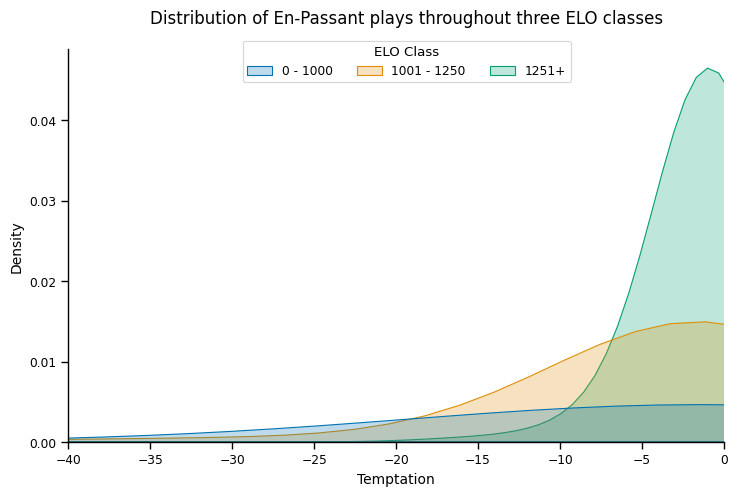
\includegraphics[width=\textwidth]{report/images/ep_distplot.png}
  \caption{Every value of temptation on the chart is negative since we assume a move cannot be better than the Stockfish evaluated best move. Values with a temptation of $0$ were excluded as the number of games where en-passant did occur if it was the best move was overwhelmingly high across every class.}
  \label{fds-project-template:fig:ep_distplot}
\end{figure*}

After plotting this graph, we tried to emulate these results by creating a new field for the probability that someone in a certain Elo would play an en-passant move. There wasn't enough samples in the dataset to get any meaningful information from comparing single values, so we rounded each player's Elo to the nearest $10$ and calculated the probability using the following formula:
$$\mathbb{P}(\text{Elo class}) = \frac{\text{Games with successful e.p. captures}}{\text{Total games with e.p. opportunity}}$$

At this point, there are $8$ parameters involved in the data, $4$ of those are categorical, i.e. the player's colour, if en-passant actually happened, if the game was rated, and the time class. The other variables being the time taken, a Stockfish evaluation of the player's actual move in the dataset, the probability of someone in their Elo class playing en-passant, and finally the temptation. We then split our dataset in a $60:40$ ratio for the training and test set respectively (Fig. \ref{fds-project-template:fig:knn}). We used this ratio because any wider a difference and the model would overfit/underfit the data [Lila work out which one it is] meaning the confusion matrix wouldn't [Lila finish this]. Using the training set, we performed a PCA analysis to reduce the dimensionality of the dataset, and then utilised a k-nearest neighbours algorithm to classify the test set.\newline

From Fig. \ref{fds-project-template:fig:ep_distplot}, we can see that higher Elo players have a very concentrated area of temptation where they will perform a capture, i.e. when the temptation is close to $0$. The drop-off after being relatively sharp, and turning to a near-zero chance for any move below $T(move)=-20$. On the other hand, both the medium and lower Elo classes have a much spread-out and shallower slope, which indicates that in lower Elos, the novelty of playing en-passant does outweigh the potential repercussions of playing a bad move. However, all three Elo classes seem to follow a normal distribution, implying it would be possible to predict how a player at a certain ELO will play given an en-passant opportunity.\newline

On the other hand, from the K-NN Chart (Fig. \ref{fds-project-template:fig:knn}), the left and right sides are somewhat defined, but the middle Elo class has a very erratic classifying area, with it being blended in with the other two classes as well. This is likely due to there being a lot of overlap from all three categories in the section where most medium Elo games lie, making it difficult to accurately classify a data point inside of that region from the parameters that we used. From these two graphs, it is clear that although we can somewhat predict the chances of an en-passant move given the Elo of a player, the inverse is not true and using only context surrounding an en-passant move is not nearly enough to predict someone's Elo without a much more accurate model and further parameters of the players involved. \newline

To further back this up, we created a confusion matrix (Table \ref{tab:confusion_matrix}) detailing the numbers of correct and incorrect predictions of the k-NN model on the test set for each Elo class. 
\begin{figure*}[t]
  \centering
  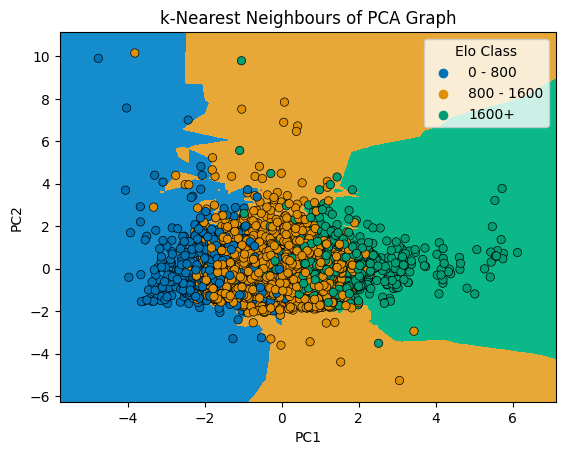
\includegraphics[width=\textwidth]{report/images/knn_graph.png}
  \caption{Each dot in the chart represents a unique player in the dataset, and their Elo is sorted into the corresponding category of Elo class. The algorithm is tuned with between 3 and 7 neighbours and picks the result with the highest accuracy, in this case 5.}
  \label{fds-project-template:fig:knn}
\end{figure*}

Values from the confusion matrix were used to calculate metrics to evaluate the model's predictive performance. These metrics were: accuracy ($0.3412$), precision ($0.3991$), recall ($0.3412$), and sample-weighted F1 score ($0.3544$). The accuracy is below $0.5$, thus demonstrating our model has poor predictive capabilities. The precision and recall scores were used in the calculation for the F1 score, which evaluates the model for precision (amount of correctly classified data points) and robustness (whether it misses a significant amount of data) \cite{MetricsToEvaluateYourML}. To account for the test set containing different proportions of each Elo class, we used the sample-weighted calculation for the F1 score. This produced an F1 score of $0.3544$ which shows a bad fit of the model to the data, implying Elo cannot be accurately predicted from the model's hyperparameters. \newline

We further produced an ROC [Lila do this and cite figure]

\begin{table}[H]
  \centering
  \caption{Confusion matrix of the test set, providing information on the number number of data points the model predicted to be in each Elo class, alongside the actual amount in each Elo class. Here Elo classes are coded as: $1: 0 - 1,000, \newline 2: 1,001 - 1,400, \newline 3: 1,401+$.}
  \label{tab:confusion_matrix}
    \begin{tabular}{lrrr}
        \toprule
        \textbf{Location}&\textbf{Predict 1}&\textbf{Predict 2}&\textbf{Predict 3}\\
        \midrule
        \textbf{Actual 1}&$10$&$ 95$&$5.3$\tabularnewline
        \textbf{Actual 2}&$ 3$&$ 40$&$5.3$\tabularnewline
        \textbf{Actual 3}&$ 0$&$ 10$&$6.3$\tabularnewline
        \hline
    \end{tabular}
\end{table}

% \begin{figure*}[t]
%   \centering
%   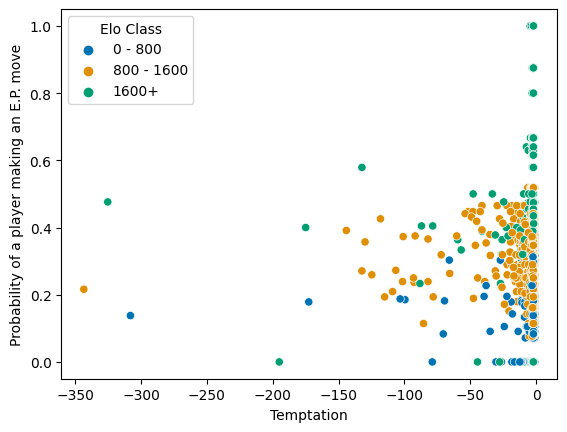
\includegraphics[width=\textwidth]{report/images/temptation_chart.png}
%   \caption{descriptive caption that i cba doing rn}
%   \label{fds-project-template:fig:temptation}
% \end{figure*}



\section{Discussion and conclusions}
% Suggested 400 words.



\paragraph{Summary of findings}
This study's findings indicate that the amount of difference in Elo between two players affects the outcome of a chess game, for games played on the online chess website Chess.com.  \newline

By focusing on the situational board state whenever an \textit{en passant} chess move was played, we developed a k-NN model to determine whether there was enough information from this context to predict the Elo of the player. However we
found insufficient evidence that a player's Elo was predictable from the context of this one move.




\paragraph{Evaluation of own work: strengths and limitations}
A caveat of using Stockfish is that since it is a live engine, without utilising significant processing power it will end up with slightly different results each time it runs. Although we have found that in most cases the data is similar, sometimes it generates a large variation in the graphs that will be shown in this study.\newline

Another limitation is that while the "quotient"  field measuring the probability of a player playing an en-passant move cannot be used backwards to predict the Elo of the player, the derivation of the value is taken from a rounding of the player's Elo. So this study is more of a proof of concept, as it cannot be viable to predict a person's Elo blind. A more viable option is to instead of grouping by similar Elo class, to group by individual players instead. However, in this dataset there is not a large enough sample to viably do this, as the mean number of games with a player is only $1.7370$, with a standard deviation of $4.0367$.

\paragraph{Comparison with any other related work}
E.g. ``Anscombe has also demonstrated that many patterns of data can
have the same correlation coefficient'' \cite{anscombe1973graphs}.

Wikipedia can also be cited but it is better if you find the original
reference it for a particular claim in the list of references on the
Wikipedia page, read it, and cite it.


\paragraph{Improvements and extensions}

The model used to predict the "temptation" of a move is very simplistic and does not consider other parameters other than the evaluations given by Stockfish. In the real world, there would be lots of other factors such as remaining time, or the fact that a human would not evaluate moves in the same way as a computer. However, in Fig. \ref{fds-project-template:fig:ep_distplot}, the results that were displayed were what we were expecting in this study. If improved and tuned better, the idea for the model could be used to analyse moves beyond just en-passant.

\end{multicols}

\printbibliography
\end{document}

% LocalWords:  lrrrrrrr ment Macduff Kemnay Ruchill FDS mc th fds
% LocalWords:  Anscombe dataset en-passant passant en